\chapter{Introduction}\label{ch:introduction}

In 1965, after the first successful flyby mission to Mars by NASA, the interest in the planet mars increased considerably because they saw lots of similarities to earth \cite{NASAChronology}.\\
In 1996 NASA sent out a surface rover on the Pathfinder mission, which was the first successful rover to drive on Mars. The rover was named Sojourner, and it spent 85 days exploring the terrain, snapping photographs, taking chemical and atmospheric samples\cite{NASASojournerPathfinder}\cite{NASAChronology}.\\
In 2018 NASA will send out the lander InSight to investigate the deep interior of Mars. This will be done with modern technology to get a better understanding of the history of Mars and advance our knowledge about rocky planets\cite{InSight}.\\
%In 2020 NASA will be sending a rover to Mars for further investigation of bacterial lifeforms.%cite

The purpose of this project is to create a robot which can map the area, make a path and avoid obstacles on its own. Furthermore, the design of the robot has to be just as durable or more than the current solutions.\\


\begin{figure}[h]
    \centering
    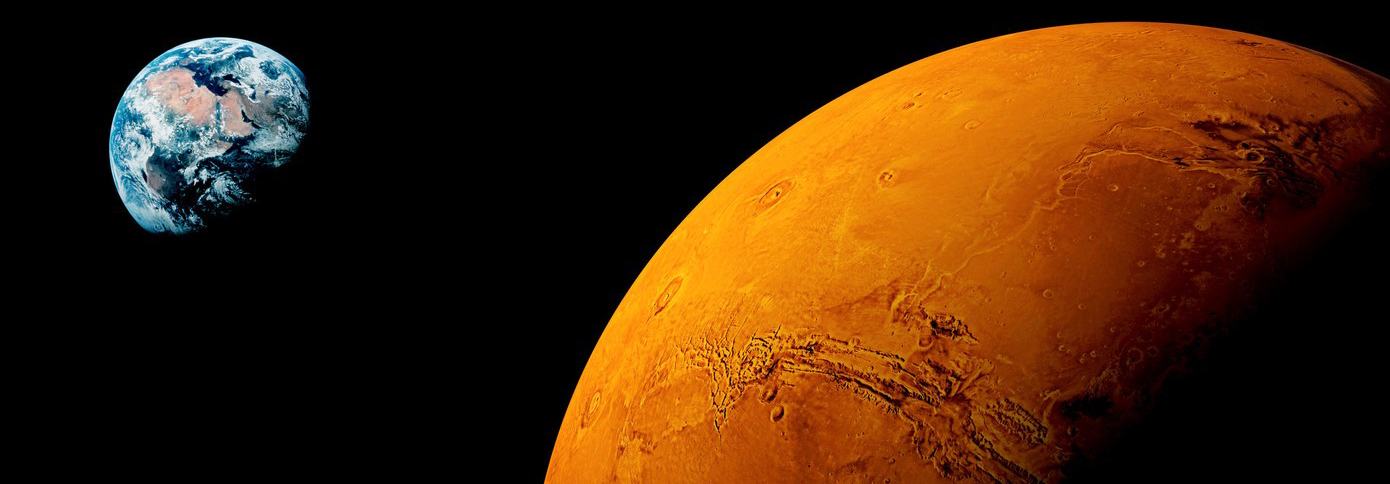
\includegraphics[width=\linewidth]{figures/639620382-mars.jpg}
    \caption{Picture of Mars and Earth\cite{MarsPics}}
    \label{fig:marsSeasons}
\end{figure}

